\documentclass{microereport}

%%%%%%%%%%%%%%%%%%%%
%%%%% Packages %%%%%
%%%%%%%%%%%%%%%%%%%%
% graphicx allows you to include images
\usepackage{graphicx}
\graphicspath{{images/}}

% booktabs adds the \toprule \midrule and \bottomrule commands
% They are used to make better looking, and more customizable, tables than
% using just \hrule
\usepackage{booktabs}

% siunitx adds the \si{} command, and allows you to easily typeset units:
% \si{\kilo\volt}
% inter-unit-product=\ensuremath{\cdot} is an option that makes it so a dot
% shows up for the product of units, instead of just writing them next to
% each other, which could lead to confusion:
% mT, is it militeslas, or tesla*meters?
\usepackage[inter-unit-product=\ensuremath{\cdot}]{siunitx}

% You won't need the lipsum package. It is used to generate filler text which
% lab reports certainly shouldn't have.
\usepackage{lipsum}

\author{Matthew Filmer}
\date{\today}
\title{Example Lab Report Format in \LaTeX{}}
\class{Introduction to Microelectronic Engineering}
\pagemark{Filmer}

\begin{document}
\maketitle
\begin{abstract}
	\lipsum[1]
\end{abstract}

\section{Introduction}
\lipsum[2-4]

\section{Theory}
\lipsum[5]
\begin{equation}
	c^2 = a^2 + b^2 - 2ab\cos\gamma
	\label{equ:lawOfCosines}
\end{equation}
\lipsum[6]
\begin{figure}
	\centering
	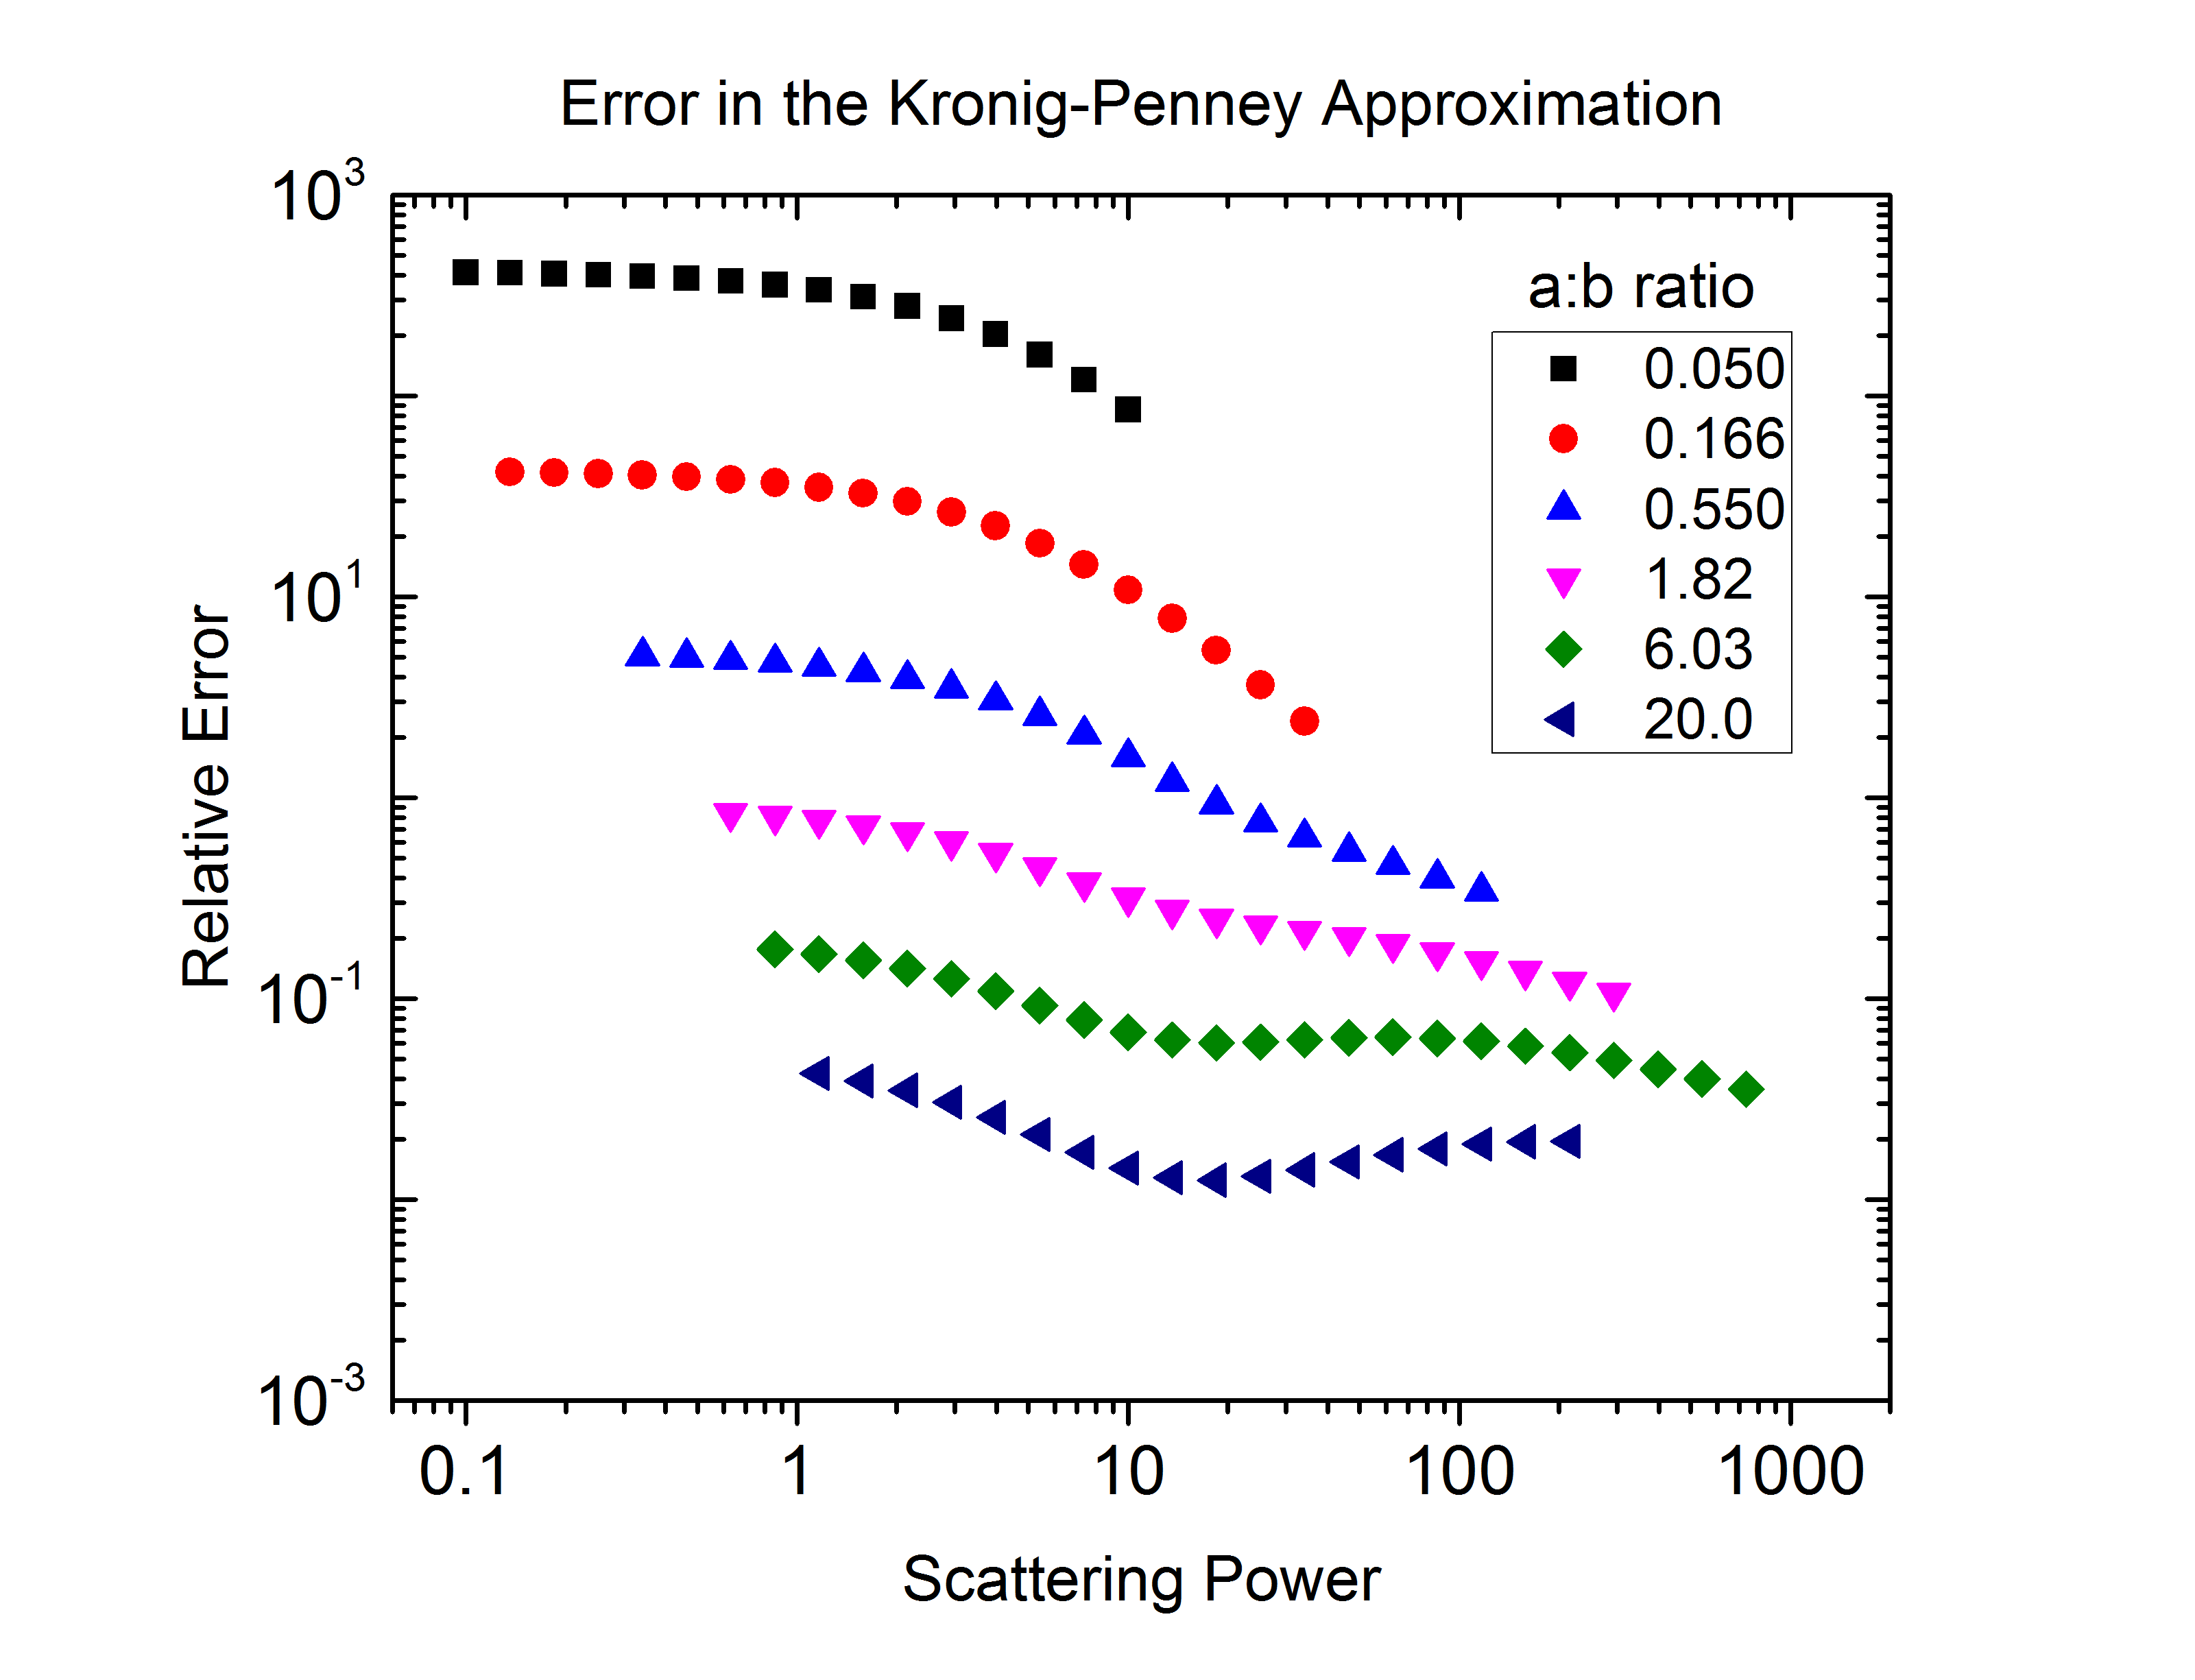
\includegraphics[width=10cm]{error}
	\caption{Your captions should be informative, and should be able to stand on their own in explaining the figure. Figures should be placed at the top or bottom of the page as to minimize breaking up the document's text. \LaTeX{} should take care of this for you though.}
	\label{fig:KPerror}
\end{figure}
\lipsum[7]

\section{Experiment}
\lipsum[8-10]
\begin{table}
	\centering
	\caption{Table captions go above the table}
	\label{tab:table}
	\begin{tabular}{ccc}
		\toprule
		Sample ID	& Velocity [\si{\meter\per\second}]	& Mass [\si{\kilo\gram}]\\
		\midrule
		A			& 982	& 17\\
		B			& 127	& 54\\
		C			& 835	& 12\\
		D			& 435	& 87\\
		\bottomrule
	\end{tabular}
\end{table}
\lipsum[11-12]

\section{Conclusion}
\lipsum[13-14]

\end{document}